\chapter{Data for incident gammas}
\label{Sec:gamma-in}

The \gettransfer\ code calculates cross sections and the integrals in
Eqs.~(\ref{Inum}) and~(\ref{Ien}) for computation of the transfer matrix
for  coherent scattering and
Compton scattering. Photoemission, pair production, and
triplet production are handled by \xndfgen.

\section{Coherent scattering}
This reaction is the result of interaction of the incident photon with all
of the electrons in the target atom and sometimes called whole-atom scattering.
There
is essentially no change in energy between the outgoing and incident
photons.  In \xendl\ instead of the energy $E$ of the incident photon, 
the data are given in terms of~$x$,
where $x$ is
\begin{equation}
  x = 
  \frac{1}{\lambda}\sin \left(
     \frac{\theta}{2} \right) =  
  \frac{1}{\lambda}
  \sqrt{\frac{1-\mulab}{2}}.
  \label{def-x}
\end{equation}
In Eq.~(\ref{def-x}) $\lambda$ is the wave length of the
incident photon given in~\AA.  Thus, in terms of the incident energy $E$, the
value of $x$ is
\begin{equation}
  x = \frac{E}{ch}\,
  \sqrt{\frac{1-\mulab}{2}}
  \label{def-x-MeV}.
\end{equation}
In \gettransfer\ the values of $x$ are scaled by $ch$,
to convert to units of energy.

The angular differential cross
section $\sigma_C(\mulab \mid E)$ takes the form
\begin{equation}
  \sigma_C(\mulab \mid E) =
    \frac{3\sigma_T}{8} (1 + \mulab^2 )
    \left \{
       [ F_F(x) + F_R(x)  ]^2 + F_I(x)^2
    \right \}.
  \label{sigma-whole-atom}
\end{equation}
where the parameter $\sigma_T$ is the classical
Thompson scattering cross section.
In Eq.~(\ref{sigma-whole-atom}) 
$F_F(x)$ is the coherent form factor, and it is a function of
$x$ in Eq.~(\ref{def-x})
The real
anomalous form factor $F_R(E)$, and the imaginary
anomalous form factor $F_I(E)$ are given in terms of
the incident energy~$E$.
The units of $\sigma_C(\mulab \mid E)$ are barns per cosine.
See the reference~\cite{ENDFB} for more information.

The reaction cross section is computed using
\begin{equation}
  \sigma( E) = \int_{-1}^1 d\mulab \, \sigma_C(\mulab \mid E).
  \label{total-sigma-whole-atom}
\end{equation}
Because the energy is assumed to be unchanged, $\Elab' = E$, and
because the gamma multiplicity is~1,
the formula Eq.~(\ref{def_pi}) for the kernel 
$K(\Elab', \mulab \mid E)$ for coherent scattering becomes
\begin{equation}
   K(\Elab', \mulab \mid E) = \sigma_C(\mulab \mid E) w(E) \delta( \Elab' - E).
  \label{K-whole-atom}
\end{equation}

For photons it is customary to use the energy-preserving transfer
matrices Eq.~(\ref{cons_en}) derived from the integrals Eq.~(\ref{Ien}),
so details are given only for the evaluation of Eq.~(\ref{Ien}).
From Eq.~(\ref{K-whole-atom}) it is seen that
\begin{equation}
    \Ien_{gh,\ell} =
     \int_{\calE_g} dE \, w(E) \widetilde \phi_\ell(E)
     \int_{\calE_h' } d\Elab' \, \int_{\mulab} d\mulab  \, 
     P_\ell ( \mulab )\, \sigma_C(\mulab \mid E)
      \, \delta( \Elab' - E) \Elab'.
  \label{Ien-whole-atom}
\end{equation}
Because both the incident particles and the outgoing particles are
photons, the outgoing energy groups $\calE_h'$ are the same as the
incident energy groups $\calE_g$.  Therefore, an integration over
$\Elab'$ in Eq.~(\ref{Ien-whole-atom}) gives the result that
$$
  \Ien_{gh,\ell} = 0 \quad \textrm{for} \quad h \ne g
$$
and
\begin{equation}
   \Ien_{gg,\ell} =
   \int_{\calE_g} dE \, w(E)  \widetilde \phi_\ell(E) E \,
   \int_{\mulab} d\mulab  \, P_\ell ( \mulab ) \sigma_C(\mulab \mid E).
  \label{Ien-whole-atom-intE}
\end{equation}

\begin{figure}
% domain of integration for whole-atom scattering
\begin{center}
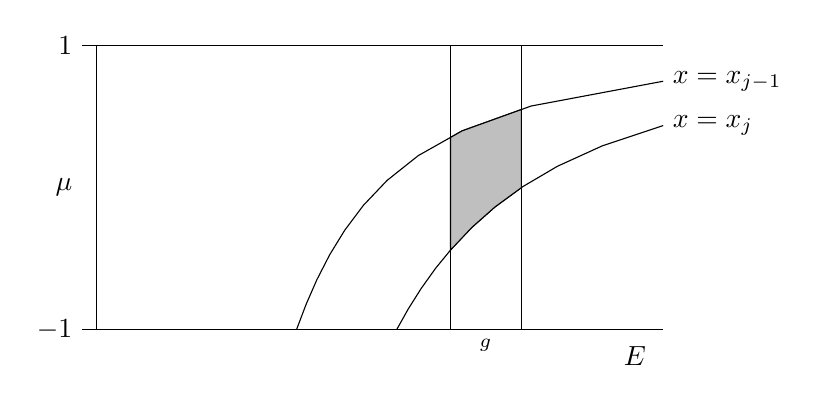
\begin{tikzpicture} [scale=1.8]
% the axes and quadrature box
  \draw(-0.1, -1) -- (4, -1);
  \draw(0, -1) -- (0, 1);
  \draw(-0.1, 1) -- (4, 1);
  \draw(2.5, -1) -- (2.5, 1);
  \draw(3, -1) -- (3, 1);
% x = constant curves
% E' = 2/sqrt{1 - mu}
\draw( 1.4142 , -1.0 ) --
( 1.4805 , -0.825 ) --
( 1.5570, -0.65 ) --
( 1.6468 , -0.475 ) --
( 1.7541, -0.3 ) --
( 1.8856, -0.125 ) --
( 2.0520, 0.05 ) --
( 2.2718, 0.225 ) --
( 2.5820, 0.4 ) --
( 3.0679, 0.575 ) --
( 4.0 , 0.75 );
% E' = 3/sqrt{1 - mu}
\draw( 2.1213, -1.0 ) --
( 2.2019, -0.85625 ) --
( 2.2925, -0.7125 ) --
( 2.3952, -0.56875 ) --
( 2.5131, -0.425 ) --
( 2.6504, -0.28125 ) --
( 2.8128, -0.1375 ) --
( 3.0094 , 0.00625 ) --
( 3.2540, 0.15 ) --
( 3.5698, 0.2938 ) --
( 4.0 , 0.4375 );
% integration region
\filldraw[fill = gray!50] (2.5000, -0.4410) --
( 2.6504, -0.28125 ) --
( 2.8128, -0.1375 ) --
(3.0000, -0.0006) --
(3.0000, 0.5505) --
( 2.5820, 0.4 ) --
( 2.5000, 0.3537) -- cycle;
% labels
  \node[left] at(-0.1, -1){$-1$};
  \node[left]  at(-0.1, 1){$1$};
  \node[left]  at(-0.1, 0){$\mu$};
  \node[below] at(2.75, -1){$\calE_g$};
  \node[below]  at(3.8, -1.05){$E$};
  \node[right] at(4, 0.75){$x = x_{j-1}$};
  \node[right]  at(4, 0.4375){$x = x_j$};
\end{tikzpicture}
\caption{Domain of integration for whole-atom scattering}
\label{Fig:coherent}
\end{center} 

\end{figure}

The domain of integration for Eq.~(\ref{Ien-whole-atom-intE}) is
shown in Figure~\ref{Fig:coherent}.  The curves for $x = x_{j-1}$ and $x = x_j$
are obtained from Eq.~(\ref{def-x-MeV}), and for $x_{j-1} \le x \le x_j$
the region of integration is bounded by these two curves and
lies within the $\calE_g$ energy bin.  This region is shaded gray in
Figure~\ref{Fig:coherent}.

\subsection{A programming detail}
Because of the $\sqrt{1 - \mulab}$ singularity in Eq.~(\ref{def-x-MeV}),
the default method for evaluating integrals with respect to $\mulab$ in 
this section is adaptive quadrature based on first-order Gaussian quadrature
for
\begin{equation}
  \int_a^b d\mulab \, F(\mulab) \sqrt{ 1 - \mulab}.
 \label{Gauss-quad-half}
\end{equation}
This method is used for integration over $\mulab$ in 
Eqs.~(\ref{total-sigma-whole-atom}) and~(\ref{Ien-whole-atom-intE}).

The default method for integration over incident energy $E$ in
Eq.~(\ref{Ien-whole-atom-intE}) is second-order adaptive Gaussian
quadrature.

\subsection{The input file for coherent scattering}
For coherent scattering, the reaction identifier in Section~\ref{data-model} 
is\\
  \Input{Process: coherent scattering}{}\\
and the data are always in the laboratory frame\\
  \Input{Product Frame: lab}{}

The quadrature methods with respect to $\mulab$ and $E$
in Eq.~(\ref{Ien-whole-atom-intE}) may be set independently
using the commands of Section~\ref{Sec:QuadratureMethods}.
The defaults are\\
    \Input{mu quadrature method:}{square root}\\
    \Input{Ein quadrature method:}{adaptive}\\
The quadrature method specified for $\mulab$ also applies to the computation of
the cross section in Eq.~(\ref{total-sigma-whole-atom}).

In \xendl\ the values of $x$ in Eq.~(\ref{def-x}) are given in units of
$\text{\AA}^{-1}$, and the \gettransfer\ code converts $x$ to energy using
the factor $ch$.  This conversion must be to the units used for the
energy bin boundaries in Sections~\ref{Ein-bins} and~\ref{Eout-bins}.
The conversion factor from $\text{\AA}^{-1}$
to energy is set as described in 
Section~\ref{Sec:cm-to-Mev}.

The value of the Thompson scattering cross section $\sigma_T$ in
Eq.~(\ref{sigma-whole-atom}) specified as discussed in
Section~\ref{Sec:Thompson-xs}.

Section~\ref{model-info} of the input file contains the information required
for calculation of the differential cross section in Eq.~(\ref{sigma-whole-atom}).
The values of the coherent form factor $F_F(x)$ are
input using\\
    \Input{Form factor: n = $n$}{}\\
    \Input{Interpolation:}{list interpolation flag}\\
followed by $n$ pairs of values of $x$ and $F_F(x)$.  The interpolation
flag is one for simple lists as in Section~\ref{interp-flags-list}.

The  real anomalous form factor $F_R(E)$ and 
imaginary anomalous form factor $F_I(E)$ are input analogously\\
    \Input{anomalous real form factor: n = $n$}{}\\
    \Input{Interpolation:}{list interpolation flag}\\
followed by $n$ pairs of values of $E$ and $F_R(E)$, and\\
    \Input{anomalous imaginary form factor: n = $n$}{}\\
    \Input{Interpolation:}{list interpolation flag}\\
followed by $n$ pairs of values of $E$ and $F_I(E)$.

An input file for coherent scattering with $x$ values to
be converted from $\text{\AA}^{-1}$ to eV
is as follows.\\
    \Input{Process: coherent scattering}{}\\
    \Input{Product Frame: lab}{}\\
   \Input{inverseWaveLengthToEnergyFactor: 12398.4190576}{}\\
    \Input{ThompsonScattering: 0.6652448}{}\\
    \Input{\# Data section}{}\\
    \Input{Form factor: n = 1272}{}\\
    \Input{Interpolation: lin-lin}{}\\
   \Input{ \indent 0.000000000000e+00  8.000000000000e+00}{}\\
 \Input{ \indent 1.000000000000e-03  8.000000000000e+00}{}\\
 \Input{ \indent 5.000000000000e-03  7.997400000000e+00}{}\\
 \Input{ \indent 6.250000000000e-03  7.995640000000e+00}{}\\
 \Input{ \indent 7.187500000000e-03  7.994550000000e+00}{}\\
   \Input{ \indent  }{$\cdots$}\\
 \Input{ \indent 1.000000000000e+09  7.999700000000e-29}{}\\
        \Input{Anomalous real form factor: n = 253}{}\\
    \Input{Interpolation: lin-lin}{}\\
    \Input{ \indent   1.000000000000e+00 -8.001506000000e+00}{}\\
   \Input{ \indent 3.000000000000e+00 -8.012308000000e+00}{}\\
    \Input{ \indent 8.367019000000e+00 -7.916407000000e+00}{}\\
    \Input{ \indent 9.300337000000e+00 -7.564924000000e+00}{}\\
   \Input{ \indent  9.624912000000e+00 -7.096145000000e+00}{}\\
   \Input{ \indent  }{$\cdots$}\\
  \Input{ \indent 1.000000000000e+07 -4.100212000000e-03}{}\\
    \Input{Anomalous imaginary form factor: n = 255}{}\\
    \Input{Interpolation: lin-lin}{}\\
    \Input{ \indent   1.000000000000e+00  0.000000000000e+00}{}\\
  \Input{ \indent3.000000000000e+00  0.000000000000e+00}{}\\
  \Input{ \indent9.030040000000e+00  0.000000000000e+00}{}\\
  \Input{ \indent9.871915000000e+00  0.000000000000e+00}{}\\
  \Input{ \indent9.913590000000e+00  3.647675000000e-01}{}\\
  \Input{ \indent9.920512000000e+00  4.548976000000e-01}{}\\
   \Input{ \indent  }{$\cdots$}\\
   \Input{ \indent1.000000000000e+07  3.311053000000e-07}{}

\section{Compton scattering}
This reaction is also called incoherent scattering, and it is
the scattering of a photon by an individual bound electron.
See the reference~\cite{ENDFB}.
The data in \xendl\ give the values
of the scattering factor $S_F(x)$ for discrete values
of the parameter $x$, defined in Eq.~(\ref{def-x})
or, equivalently, in Eq.~(\ref{def-x-MeV}).  

The angular differential cross section for Compton scattering,
$\sigma_I(\mulab \mid E)$,
depends on the ratio, $\kappa$, of the energy, $E$, of the incident photon
to the rest mass, $m_e$, of the electron,
\begin{equation}
  \kappa = \frac{E}{m_e}.
  \label{Compton-relative-E}
\end{equation}
In terms of $\kappa$ and $x$, the Compton differential cross section is
\begin{equation}
  \sigma_I(\mulab \mid E) =
    \frac{3 \sigma_T S_F(x)}{ 8[ 1 + \kappa(1 - \mulab)]^2 }
    \left[
      1 + \mulab^2 + \frac{\kappa^2 (1 - \mulab)^2}{1 + \kappa(1 - \mulab)}
    \right].
  \label{Compton-xs}
\end{equation}
Here, $\sigma_T$ is again the Thompson scattering coefficient, and the
units of $\sigma_I(\mulab \mid E)$ are barns per unit cosine.
In Eq.~(\ref{Compton-xs}) the scattering factor $S_F(x)$ accounts
for the deviation from the Klein-Nishina formula due to the fact
that the electrons are bound.
Just as for coherent scattering, the cross section for Compton
scattering is given by
\begin{equation}
  \sigma( E) = \int_{-1}^1 d\mulab \, \sigma_I(\mulab \mid E).
  \label{Compton-sigma}
\end{equation}

The calculation in \gettransfer\ of the energy $\Elab'$ of the outgoing photon
from Compton scattering is actually inconsistent.  On the one hand, the formula
Eq.~(\ref{Compton-xs}) for the differential cross section takes
into account the fact that the scattering is from bound electrons.
For the computation of $\Elab'$, however,
the approximation is made that the electron is
initially free and stationary.
This is a discrete two-body reaction,
and conservation of energy and momentum yields the result that
\begin{equation}
  \Elab' = \frac{E}{1 + \kappa(1 - \mulab)}.
  \label{Compton-Eout}
\end{equation}
Therefore, for Compton scattering the kernel $K(\Elab', \mulab \mid E)$ 
in Eq.~(\ref{def_pi}) takes the form
\begin{equation}
   K(\Elab', \mulab \mid E) = w(E) \sigma_I(\mulab \mid E) \,
     \delta\left(
         \Elab' - \frac{E}{1 + \kappa(1 - \mulab)}
     \right).
  \label{K-Compton}
\end{equation}

Upon inserting the kernel Eq.~(\ref{K-Compton}) into Eq.~(\ref{Ien}),
the computation of energy-preserving transfer matrices
for Compton scattering requires evaluation of the integrals
\begin{multline}
    \Ien_{gh,\ell} =
     \int_{\calE_g} dE \,  w(E)
     \int_{\calE_h' } d\Elab' \, \int_{\mulab} d\mulab  \, 
     P_\ell ( \mulab ) \, \sigma_I(\mulab \mid E)
      \widetilde \phi_\ell(E) \\
      \delta \left(
         \Elab' - \frac{E}{1 + \kappa(1 - \mulab)}
     \right)\Elab'.
  \label{Ien-Compton}
\end{multline}
After integrating over $\Elab'$, it is found that
\begin{equation}
    \Ien_{gh,\ell} =
     \int_{\calE_g} dE \, E  w(E) \widetilde \phi_\ell(E) \,
     \int_{\mulab} d\mulab  \,  
         \frac{P_\ell ( \mulab ) \sigma_I(\mulab \mid E)}{1 + \kappa(1 - \mulab)}.
  \label{Ien-Compton-intE}
\end{equation}
As in coherent scattering, the default quadrature method for integration
with respect to $\mulab$ in Eqs.~(\ref{Compton-sigma}) and~(\ref{Ien-Compton-intE})
is first-order 
Gaussian quadrature for the weighted integral Eq.~(\ref{Gauss-quad-half}).

\begin{figure}
% domain of integration for Compton scattering
\begin{center}
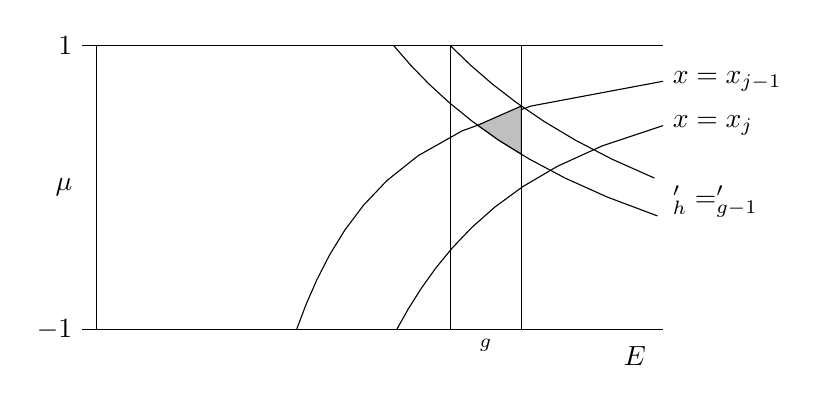
\begin{tikzpicture} [scale=1.8]
% the axes and quadrature box
  \draw(-0.1, -1) -- (4, -1);
  \draw(0, -1) -- (0, 1);
  \draw(-0.1, 1) -- (4, 1);
  \draw(2.5, -1) -- (2.5, 1);
  \draw(3, -1) -- (3, 1);
% x = constant curves
% E' = 2/sqrt{1 - mu}
\draw( 1.4142 , -1.0 ) --
( 1.4805 , -0.825 ) --
( 1.557 , -0.65 ) --
( 1.6468 , -0.475 ) --
( 1.7541 , -0.3 ) --
( 1.8856, -0.125 ) --
( 2.052 , 0.05 ) --
( 2.2718 , 0.225 ) --
( 2.582 , 0.4 ) --
( 3.0679, 0.575 ) --
( 4.0 , 0.75 );
% E' = 3/sqrt{1 - mu}
\draw( 2.1213 , -1.0 ) --
( 2.2019 , -0.85625 ) --
( 2.2925, -0.7125 ) --
( 2.3952 , -0.56875 ) --
( 2.5131 , -0.425 ) --
( 2.6504 , -0.28125 ) --
( 2.8128 , -0.1375 ) --
( 3.0094 , 0.00625 ) --
( 3.254 , 0.15 ) --
( 3.5698 , 0.29375 ) --
( 4.0 , 0.4375 );
% outgoing energy bin
\draw( 3.9388, 0.0667 ) --
( 3.6396, 0.2 ) --
( 3.3826 , 0.3333 ) --
( 3.1595 , 0.4667 ) --
( 2.9640 , 0.6 ) --
( 2.7913 , 0.7333 ) --
( 2.6376, 0.8667 ) --
( 2.5 , 1.0 );
\draw( 3.9598, -0.2 ) --
( 3.6050, -0.06667 ) --
( 3.3086, 0.06667 ) --
( 3.0573, 0.2 ) --
( 2.8414 , 0.3333 ) --
( 2.654, 0.4667 ) --
( 2.4898, 0.6 ) --
( 2.3447 , 0.7333 ) --
( 2.2156, 0.8667 ) --
( 2.1 , 1.0 );
% quadrature region
\filldraw[fill = gray!50]  (2.6920, 0.4396) --
(3.0000, 0.5755) --
(3.0000, 0.2354) --
(2.8414 , 0.3333 ) -- cycle;
% labels
  \node[left] at(-0.1, -1){$-1$};
  \node[left]  at(-0.1, 1){$1$};
  \node[left]  at(-0.1, 0){$\mu$};
  \node[below] at(2.75, -1){$\calE_g$};
  \node[below]  at(3.8, -1.05){$E$};
  \node[right] at(4, 0.75){$x = x_{j-1}$};
  \node[right]  at(4, 0.4375){$x = x_j$};
  \node[right]  at(4, -0.1){$\calE'_h = \calE'_{g-1}$};
\end{tikzpicture}
\caption{Domain of integration for Compton scattering}
\label{Fig:Compton}
\end{center} 

\end{figure}

Because of the relation Eq.~(\ref{Compton-Eout}) between the energies
of the incident and outgoing photons, the range of integration in 
Eq.~(\ref{Ien-Compton-intE}) has an extra degree of complexity in
comparison with Eq.~(\ref{Ien-whole-atom-intE}).  In particular,
the presence of the 
$\delta$-function in Eq.~(\ref{Ien-Compton}) constrains $E$ and
$\mulab$ so that $\Elab'$ is in the $\calE_h'$ energy bin.  Figure~\ref{Fig:Compton}
shows the geometry in the case of down-scattering by one
energy group, $\calE_h' = \calE'_{g-1}$.  In Figure~\ref{Fig:Compton} the curves
delimiting the $\calE_h'$ were obtained by rewriting the energy
condition Eq.~(\ref{Compton-Eout}) in the form
$$
  E = \frac{\Elab'}{1 - (1 - \mulab)\Elab'/m_e}
$$
and taking the top and bottom of the
$\calE_h'$ energy bin as values of~$\Elab'$.  The range of integration in
Eq.~(\ref{Ien-Compton-intE}) is the overlap of the three regions
(1) that determined by the interval $x_i \le x \le x_{i+1}$
of scattering factor data values,
(2) the incident energy bin $E$ in $\calE_g$, and
(3) the outgoing energy bin $\Elab'$ in $\calE_h'$.

\subsection{The input file for Compton scattering}
The reaction identifier in Section~\ref{data-model} for
Compton scattering is\\
  \Input{Process: Compton scattering}{}\\
and the data is always in the laboratory frame\\
  \Input{Product Frame: lab}{}

This default quadrature methods with respect to $\mulab$ 
and $E$ in Eq.~(\ref{Ien-Compton-intE}) are\\
    \Input{mu quadrature method:}{square root}\\
    \Input{Ein quadrature method:}{adaptive}\\
The quadrature method specified for $\mulab$ also applies to the computation of
the cross section in Eq.~(\ref{Compton-sigma}).  It is possible
to override these choices as explained in
Section~\ref{Sec:QuadratureMethods}.

As in coherent scattering, the values of $x$ used for Compton
scattering in \xendl\ are in units of $\text{\AA}^{-1}$, so these are
converted to energy units as in Section~\ref{Sec:cm-to-Mev}.  This
conversion must be to the units used for the energy bin boundaries in
Sections~\ref{Ein-bins} and~\ref{Eout-bins}.

Specification of the Thompson scattering cross section $\sigma_T$
in Eq.~(\ref{Compton-xs}) is as in Section~\ref{Sec:Thompson-xs}.
The value $m_e$ of the rest mass of the electron used in
Eq.~(\ref{Compton-relative-E}) is set as
in Section~\ref{Sec:electron-mass}, and it must be given
in the units used for the energy bin boundaries.

Section~\ref{model-info} of the input file contains the value of the
scattering factor $S_F(x)$ for various values of~$x$.  The format is\\
    \Input{ScatteringFactorData: n = $n$}{}\\
    \Input{Interpolation:}{list interpolation flag}\\
followed by $n$ pairs of values of $x$ and $S_F(x)$.    The interpolation
flag is one for simple lists as in Section~\ref{interp-flags-list}.

An input file for Compton scattering with units of $x$
to be converted from $\text{\AA}^{-1}$ to eV is as follows.\\
    \Input{Process: Compton scattering}{}\\
    \Input{Product Frame: lab}{}\\
   \Input{inverseWaveLengthToEnergyFactor: 12398.4190576}{}\\
    \Input{ThompsonScattering: 0.6652448}{}\\
    \Input{Electron mass: 511000}{}\\
    \Input{ScatteringFactorData: n = 453}{}\\
    \Input{Interpolation: lin-lin}{}\\
     \Input{ \indent 0.000000000000e+00  0.000000000000e+00}{}\\
  \Input{ \indent 1.000000000000e-07  1.100000000000e-12}{}\\
  \Input{ \indent 1.059602649007e-07  1.235033551160e-12}{}\\
  \Input{ \indent 1.126760563380e-07  1.396548303908e-12}{}\\
  \Input{ \indent 1.163636363636e-07  1.489454545455e-12}{}\\
\Input{ \indent }{$\cdots$}\\
 \Input{ \indent 1.000000000000e+09  8.000000000000e+00}{}
 
